\section{Transform}

In order to explain our algorithm consider the following notation: $i$ refers to the $i-th$ frame in the original video, and $i'$ refers to the $i-th$ frame in the stabilized video.

Initially, we considered the following algorithm to compute $i'$:
\begin{enumerate}
	\item extract keypoints($X$) from $(i-1)'$
	\item extract keypoints($Y$) from $i$
	\item find matches($M$) between $X$ and $Y$
	\item compute transformation $T$ from $M$.
	\item apply transformation $T$ to $i$
\end{enumerate}

With this approach, we were obtaining a lot of transformations errors(figure \ref{fig:misstransformations}) because the differences between $i$ and $(i-1)'$ are complex. Thus we defined anothe approach:   

\begin{figure}[!h]
	\centering
	\begin{subfigure}{0.5\textwidth}
	  \centering
	  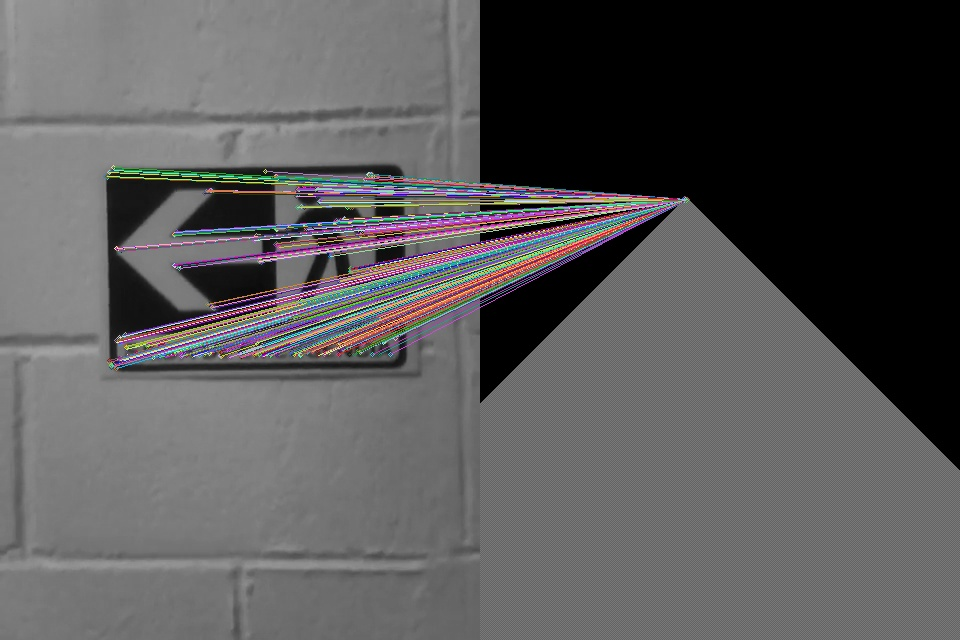
\includegraphics[width=0.8\linewidth]{figs/mistrans01.jpg}
	\end{subfigure}%
	\begin{subfigure}{0.5\textwidth}
	  \centering
	  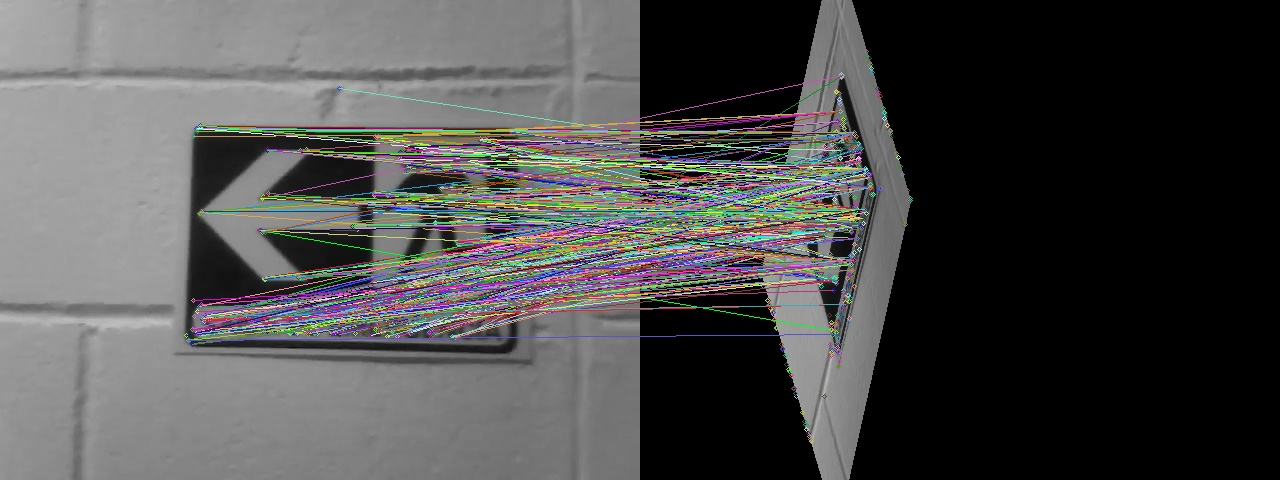
\includegraphics[width=0.8\linewidth]{figs/mistrans02.jpg}
	\end{subfigure}%
	 \caption{Errors of transformation using initial approach}
	\label{fig:misstransformations}
\end{figure}

\begin{enumerate}
	\item extract keypoints($X$) from $i-1$
	\item transform keypoints location of $i-1$ based on $(i-1)'$
	\item extract keypoints($Y$) from $i$
	\item find matches($M$) between $X$ and $Y$
	\item compute transformation $T$ from $M$.
	\item apply transformation $T$ to $i$
\end{enumerate}

We assume that the difference between adjacent frame in the original video is small. Thus, we compare the feature vector of $i$ and $i-1$, but the keypoints location of $i$ and $(i-1)'$.

Once we have the transformation of parameters we apply it for every pixel in $i$, depending of the movement, some black holes and lines appears(Figure \ref{fig:diff-interpolation}). Thus, we interpolate this points with the average of four neighbors and fill with zero the cases when the neighbors are also empty.

\begin{figure}[!h]
	\centering
	\begin{subfigure}{0.5\textwidth}
	  \centering
	  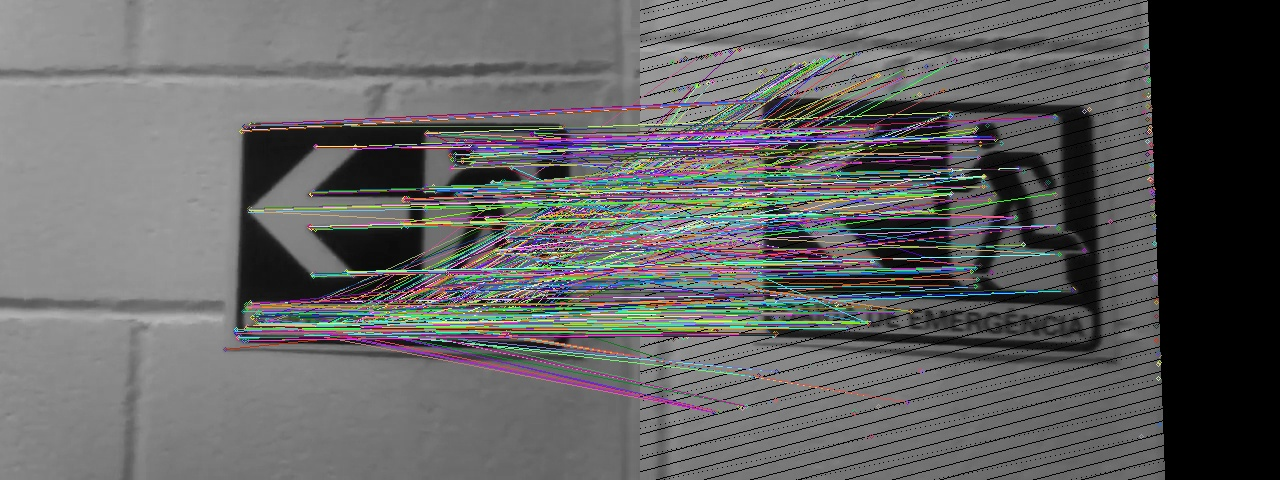
\includegraphics[width=0.8\linewidth]{figs/without-interpolation.jpg}
	  \caption{Without interpolation}
	\end{subfigure}%
	\begin{subfigure}{0.5\textwidth}
	  \centering
	  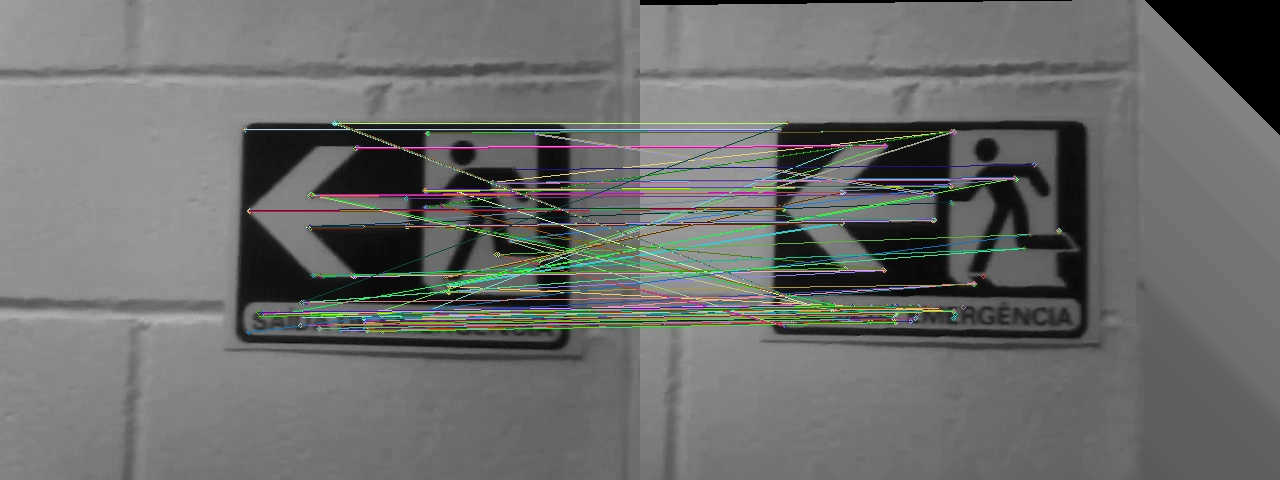
\includegraphics[width=0.8\linewidth]{figs/with-interpolation.jpg}
	  \caption{With interpolation}
	\end{subfigure}%
	 \caption{Comparison of results fof transformation uisng interpolation}
	\label{fig:diff-interpolation}
\end{figure}



result

L2-NORM
	VID0
	54.4464731615812
	24429436.7665
	VID1
	37.321051031466155
	29964112.0618
	VID2
	54.4464731615812
	24429436.7665

30-12 Orb
	VID0 fram 1
	43.35933494567871
	2330901497.0
	VID1 frame 11
	29.774162249131635
	89788339.9091
	VID2 frame 3
	22.77377374966939
	1185961909.67

NMS TRUE
	VID0 frame 37
	15.791857308811611
	42818733.9444
	VID1 frame 1
	16.9178147315979
	2531291808.0
	VID2 frame 14
	13.706815736634391
	194895992.714

S 200
	VID0
	62.691284131277634
	24540916.1218
	VID1
	42.43146139866597
	29430481.3977
	VID2
	45.6238714792196
	28768129.3107

S 100
	VID0
	64.32794978775954
	24672510.2183
	VID1
	42.98294043633008
	30052053.0116
	VID2
	45.26221292227217
	44096547.9223


S 36
	VID0
	62.32433629156974
	25921522.7817
	VID1 frame 205
	43.00332358523113
	44613346.3756
	VID2 frame 14
	46.593267457825796
	135858245.357
